\documentclass[journal]{IEEEtran}

\usepackage{mathtools}
\usepackage{amssymb}
\usepackage{amsmath}
\usepackage{hyperref}
\usepackage{breqn}
\usepackage{graphicx}
\usepackage{float}
\usepackage{listings}
\usepackage{setspace}
\usepackage{xcolor}
\usepackage{subcaption}

\usepackage{algpseudocode}
\usepackage{algorithm}

\algnewcommand\algorithmicforeach{\textbf{for each}}
\algdef{S}[FOR]{ForEach}[1]{\algorithmicforeach\ #1\ \algorithmicdo}

\definecolor{mygray}{gray}{0.7}
\newcommand{\commentsymbol}{//}% or \% or $\triangleright$
\algrenewcommand\algorithmiccomment[1]{\hfill \commentsymbol{} #1}
\makeatletter
\newcommand{\LineComment}[2][\algorithmicindent]{\Statex \hspace{#1}{\color{mygray}\commentsymbol{} #2}}
\makeatother
\newcommand{\varfont}{\texttt}

\DeclareMathOperator*{\argmax}{arg\,max}
\DeclareMathOperator*{\argmin}{arg\,min}

% ceil/floor
\def\lc{\left\lceil}
\def\rc{\right\rceil}
\def\lf{\left\lfloor}
\def\rf{\right\rfloor}

% given
\newcommand\given[1][]{\:#1\vert\:}

% eggplant
\DeclareRobustCommand{\eggplant}{%
  \begingroup\normalfont
  %\includegraphics[height=\fontcharht\font`\B]{eggplant_1f346.png}%
  \endgroup
}

% skull
\DeclareRobustCommand{\skull}{%
  \begingroup\normalfont
  %\includegraphics[height=\fontcharht\font`\B]{skull_1f480.png}%
  \endgroup
}
% multi-line equations
\usepackage{breqn}

%algorithms
%\SetKwInput{KwInput}{Input}                % Set the Input
%\SetKwInput{KwOutput}{Output}              % set the Output

% correct bad hyphenation
%\hyphenation{op-tical net-works semi-conduc-tor}

\begin{document}
\title{Sensor Bias Estimation and Compensation for Practical Multisensor-Multitarget Tracking}
\author{David~Schonborn, T.~Kirubarajan, R.~Tharmarasa}
\maketitle


% For editing purposes
%\onecolumn
%\setstretch{3}





\begin{abstract}
Estimating and compensating for sensor biases are essential in multisensor-multitarget tracking scenarios, where association of tracks or measurements originating from different sensors is required. Ignoring measurement bias can cause data association to fail and result in substantial performance degradation. Many approaches to estimate and compensate for biases exist, but can only be used under specific operational conditions. In contrast to the assumptions of existing literature, practical sensor networks often operate under demanding conditions including a distributed fusion architecture, time-varying bias, multiple heterogeneous sensors with nonlinear measurement models, limited availability of computational resources, and asynchronous communication without full availability. By restructuring the estimation problem to avoid sources of inconsistency and leveraging flexible tools such as the Unscented Transform and Covariance Intersection, this paper proposes a computationally efficient bias estimation algorithm that can be applied to a broad range of realistic scenarios. Results are presented for a simulated application in multisensor-multitarget terrain-aided video tracking to evaluate the proposed algorithm. These results demonstrate its effectiveness in reducing bias-compensated track RMSE to levels comparable to those of unbiased sensors. This general bias estimation algorithm can be implemented in a wide range of practical systems without significant modification.

\end{abstract}
\IEEEpeerreviewmaketitle








\section{Introduction} \label{introduction}
In multisensor-multitarget tracking the objective is to estimate the state (position, velocity, etc.) of targets using information obtained from multiple sensors. In many practical systems these sensors are subject to two types of measurement errors. The first is zero-mean noise which can be removed effectively through filtering (for example, using a Kalman Filter) \cite{kalman1960new}. The other type of error is bias which is constant or slowly-varying over time, not zero-mean, and can not always be removed through standard filtering processes \cite{bar2004estimation}. Although bias can negatively affect estimation performance in any tracking problem, it is particularly problematic in multisensor-multitarget tracking where association of measurements or tracks from different sensors is required. This degraded performance can take the form of missed or wrong associations \cite{TODO}, formation of ghost tracks \cite{TODO}, decreased track accuracy \cite{TODO}, inconsistent tracks \cite{TODO}, and decreased track probability of detection \cite{TODO}. This motivates the development of algorithms to estimate and compensate for bias errors prior to fusion.

Realistic operational conditions often involve additional challenges such as using a specific fusion architecture, time-varying measurement bias, imperfect knowledge of sensor positions, highly nonlinear measurement models, heterogeneous sensors, heterogeneous state space, targets moving in varied terrain, reduced communication bandwidth or unreliable communication, limitations in computation power, a large (possibly time-varying) number of sensors, or asynchronous data updates. There are many approaches to bias estimation to be found in the existing literature, some that are even optimal under certain conditions, but most address only a subset of the realistic challenges faced by many practical systems. Furthermore, many largely-speaking practical methods are only applicable to certain specific scenarios, making applications to large, heterogeneous sensor networks an exercise in patchwork.

Bias estimation and compensation methods in the existing literature can be broadly divided into three categories. There are methods that use an augmented state vector to simultaneously estimate the state of all targets and sensor biases, others that formulate a pseudomeasurement of the sensor biases that is independent of the target state, and finally those that employ particle methods to estimate various states including sensor biases. Each of these categories is reviewed below with a summary of their strengths and limitations.

Several methods have been proposed to estimate sensor biases by creating an augmented (or stacked) state vector and using, for example, a Kalman Filter (KF) to jointly estimate the states of the targets and sensor biases \cite{van1993systematic, friedland1969treatment, yi2019exactly}. In the literature these methods are frequently referred to as Augmented State Kalman Filter (ASKF) methods. Under certain conditions these methods are able to produce an optimal solution \cite{van1993systematic, yi2019exactly}. However, if all these state variables are stacked, this can result in a very large state vector if the scenario involves many sensors, targets, and/or bias parameters. Since the KF requires inversion of the covariance matrix, which has computational complexity of approximately $\mathcal{O}(n^3)$ (where $n$ is the state dimension), this can become computationally prohibitive for use in a real time system \cite{van1993systematic}. Related methods have been proposed which decouple the state vector in various ways, allowing for the use of several KFs of smaller dimension instead of a single larger one, reducing the computational load. In \cite{van1993systematic, kastella2000bias} approximations are used to decouple the augmented state, but are subject to performance degradation. In \cite{yi2019exactly} an exact formulation is proposed to decouple the augmented state, allowing the use of multiple KFs for different targets, each one stacked with the sensor bias estimates. Using their approach the state vector of each KF still grows with the number of sensors, so for large sensor networks this can become computationally expensive. A two-stage approach was proposed in \cite{friedland1969treatment} to decouple the target states from the sensor biases when the biases are constant, which was extended by \cite{alouani1992two} to accommodate dynamic biases with white or coloured Gaussian noises. However \cite{alouani1992two} also point out that this approach is only equivalent to the ASKF under a restrictive constraint which is not usually satisfied in practice. Additionally, most ASKF algorithms operate under the assumption that all measurements from the sensors are available at the fusion center, and that these measurements are synchronized in time \cite{van1993systematic, yi2019exactly, alouani1992two}. This makes them only applicable to time-synchronized centralized fusion networks. Extension to nonlinear systems is possible through linearization, for example using the Extended Kalman Filter (EKF), but these require situational derivations and are still sub-optimal \cite{bar2004estimation}. For highly nonlinear systems it may be desirable to use a robust tool such as the Unscented Transform (see section \ref{unscentedtransform}), and these ASKF methods are not directly extensible to accommodate this.

Another popular approach is to formulate a pseudomeasurement of the sensor biases that is independent of the target state by taking the difference between measurements or tracks from different sensors such that the target state cancels out \cite{taghavi2016practical, taghavi2020geo, song2021efficient, zhu2015joint}. This leaves just a noisy measurement of the sensor biases that can be used to estimate the biases directly. This strategy has been successfully employed in various fusion architectures \cite{song2021efficient, taghavi2020geo, zhu2015joint, taghavi2016practical} and with asynchronous data rates \cite{taghavi2016practical, yong2016asynchronous}. In most cases the state vector for bias estimation is the stacked vector of the biases from the sensors used to formulate the pseudomeasurement, so it is much more computationally efficient than the ASKF which also stacks all the target states. This state vector still grows with the number of sensors, so for large sensor networks it can still become computationally expensive. Beyond just computational load, many of these methods are limited to use with a pair of sensors \cite{song2021efficient, taghavi2020geo, yong2016asynchronous} so use with a large sensor network is not possible without the additional consideration of pairing sensors. Some methods, such as \cite{taghavi2016practical}, present computationally efficient solutions with multiple sensors under specific circumstances. Another challenge with pseudomeasurement methods lies in their application to heterogeneous sensor networks. For different sensor types (or different bias models), different formulations are needed and often lead to different solution methodologies. For example, in \cite{taghavi2016practical} a system with radar sensors is considered and can be solved using Recursive Least Squares (RLS) or a KF (for constant and time-varying biases, respectively). In \cite{taghavi2020geo} a similar starting point is taken but applied to a pair of video sensors, and the resulting solution requires minimizing a nonlinear cost function using the genetic algorithm (although in \cite{song2021efficient} an alternative method is proposed that applies approximations allowing RLS to be used). Finally, highly nonlinear systems remain a challenge in a similar way as with the AKSF methods. There are solutions that can be applied, frequently using a converted measurement model \cite{taghavi2016practical, taghavi2020geo, song2021efficient}, but requires situational modelling of the bias in the converted measurement model. It may be more desirable for practical implementation purposes in a heterogeneous network if a unified approach could be applied in terms of solution methodology across different models of the measurement and biases.

The final category of methods that have been applied to bias estimation are those that use particle methods such as the particle filter and other related methods that use a number of (usually weighted) particles to represent the distribution of the variables of interest. These approaches are very flexible in handling situations with nonlinear systems or non-Gaussian distributions, but there are also some major drawbacks. The computational load can be substantial, especially if the state space dimension is large, since enough particles must be used to achieve adequate coverage and this number grows exponentially in the number of dimensions. Strategies can be used to reduce the sampling dimension, such as in Rao-Blackwellised Particle Filters (RBPFs) where some of the variables of the augmented state are marginalized out, for example in \cite{li2003parameter}. However if the number of dimensions that are decidedly required in the state remains large (for example if there are many bias parameters), the problem persists. In addition to this, particle filters are known to suffer from the problems of degeneracy and sample impoverishment \cite{gordon2004beyond}. The degeneracy problem refers to the tendency for a large number of particles to have near-zero weights as the filter is updated, requiring a large amount of computational power to be spent updating these particles that are not very relevant to the distribution estimate \cite{gordon2004beyond}. Degeneracy can be partly solved by resampling, where samples are redrawn to have equal weights but still represent approximately the same distribution \cite{gordon2004beyond}. However this introduces a tuning parameter to set a degeneracy threshold for when resampling should occur, and can also result in worsened sample impoverishment \cite{gordon2004beyond}. Sample impoverishment refers to the problem of having many samples which represent either very similar points or the same points, resulting in low sample diversity. This problem is especially prominent when process noise is low, or zero as in the case of constant biases \cite{gordon2004beyond}. Approaches have been proposed counteract sample impoverishment by adding some artificial process noise to static parameters \cite{liu2001combined, gellert2018parameter} but this introduces at least one additional tuning parameter.

Another important aspect of the sensor registration problem is bias compensation. Many existing works simply assume the bias estimate to be sufficiently accurate to correct the bias, and treat the problem of bias compensation by simply adjusting the measured values by subtracting the mean of the estimated bias, assuming the bias estimates to be sufficiently accurate (for example, in \cite{song2021efficient}). In \cite{ying20103d} a bias compensation method accounting for the covariance of the bias estimate was proposed and found to produce more accurate tracks when compared with the simple approach considering only the mean. This suggests that it is not always reasonable to ignore the uncertainty of the bias estimate during bias compensation. The method from \cite{ying20103d} requires explicit modeling of the cross-covariance terms in the update step and simplifies them with some approximations (including approximating the cross-covariance between the bias estimate and the state estimate as zero). For methods that perform joint estimation of the states and biases (such as the full ASKF) this is not an issue since these terms are maintained already, but these remain subject to other restrictions (as described above). See section \ref{biascompensation} for more information about bias compensation approaches.

Given the limitations of existing methods discussed above, there remains a need for a unified, flexible bias estimation method that can be applied to large, heterogeneous sensor networks without significant limitations in terms of the fusion architecture, the arrival of incoming data, computational feasibility, measurement and bias model, or state space model. In this paper a novel algorithm for sensor bias estimation is presented to address this need. Section \ref{background} provides necessary the background on existing algorithms that are used within the proposed algorithm and simulated scenario. A mathematical formulation of the general problem is given in section \ref{problemstatement} that introduces the relevant notations and concepts. Section \ref{proposedalgorithm} describes the proposed algorithm for bias estimation in detail, along with a discussion of bias compensation and a computational complexity analysis. An example application with required implementation details and corresponding simulation results are presented in section \ref{simulationresults}. Section \ref{discussion} discusses these results, their implications, and limitations of the proposed algorithm. A conclusion summarizes the findings of this work in section \ref{conclusion}.

\section{Background} \label{background}

\subsection{Multisensor-Multitarget Tracking}
In multisensor-multitarget tracking problems, a number of sensors are used to track multiple targets (estimate their state, for example their position and velocity). In the general case, both the number of sensors and the number of targets may be time-varying. First, sensors measure the target state according to a measurement model. A general model for a sensor measurement $z$ of (true) target state $x$ at time index $k$ is given in equation \ref{eq:generalmeasurementmodel}. The general measurement model includes a vector of bias parameters $\beta$ that may be constant or time-varying, and measurement noise $w$. The measurement noise is typically assumed zero-mean with covariance $R$ and independent between different measurements (not auto-correlated over time) \cite{bar2004estimation}. The function $h$ maps the true measured state and bias parameters to the measurement space.

\begin{equation}
    z(k) = h(x(k), \beta(k)) + v(k) \\
\label{eq:generalmeasurementmodel}
\end{equation}

Each measurement is usually assumed to correspond to a single target, and each sensor is assumed to provide at most one measurement for each target at a single instance in time. These measurements are used to initialize and maintain estimates of the states of targets over time, a process known as filtering. In addition to the measurement model, filtering requires a model of how the target state evolves over time, referred to as a state-transition model \cite{bar2004estimation}. In tracking applications this is often given in the form of a kinematic model. A general state-transition model is given in equation \ref{eq:generalsystemmodel} where $f$ is a function that maps the target state $x(k)$ at time $k$ to the target state $x(k+1)$ at time $k+1$. The second argument to the function $f$ indicates that this function may be time-varying. The transition is also subject to process noise $w$, which typically is assumed to be Gaussian, zero-mean with covariance $Q$, and independent over time \cite{bar2004estimation}. Some formulations of the state-transition model also include modeling of a known control input, but for non-cooperative tracking this cannot be assumed known and is not included here.

\begin{equation}
    x(k+1) = f(x(k), k+1) + w(k+1) \\
\label{eq:generalsystemmodel}
\end{equation}

In the case of independent zero-mean Gaussian noises, zero measurement bias, and linear models for both the measurement and system, the optimal estimator (in terms of minimum mean-squared error) is the Kalman Filter (KF) \cite{bar2004estimation}. The KF can be implemented efficiently using a recursive formulation, so it is very practical for online applications. Many practical applications do not conform exactly to the optimality requirements of the KF, but none the less it remains the most popular choice as the basis of many tracking systems. Extensions to the KF, such as the Extended Kalman Filter (EKF) \cite{bar2004estimation} and Unscented Kalman Filter (UKF) \cite{julier1997new}, exist and have proven successful (through numerous applications) in expanding the scope of operation of the Kalman Filter framework. Due to the ubiquity of the KF framework, it is desirable for solutions to various tracking problems be compatible with its use. This compatibility is often achieved through linearization of a nonlinear measurement function (as in the EKF) or through a Gaussian approximation of a random variable (as in the UKF).

When using multiple sensors it becomes necessary to combine (or fuse) their information. There are three main types of fusion architecture that define how information is combined from different sources. These architectures will be reviewed here briefly in terms of their relevant aspects, but for a more thorough treatment the reader is referred to \cite{castanedo2013review}. In centralized fusion architectures, each sensor sends all its measurements back to the central fusion center (CFC) where information is combined at the measurement level (measurement-to-track fusion) \cite{castanedo2013review}. In practical systems a centralized fusion architecture often presents challenges in terms of communication bandwidth, with all sensors needing to transmit all measurements to the CFC to perform fusion \cite{castanedo2013review}. To address this, a distributed fusion architecture can be used. In a distributed architecture, information from measurements is processed into tracks at the local sensor node before transmission to the CFC where the tracks are combined through track-to-track fusion \cite{castanedo2013review}. Transmitting tracks instead of measurements can relax the requirement that communication takes place at every local sensor update and reduce overall bandwidth requirements, but introduces the challenge of fusing correlated information \cite{castanedo2013review}. There is also a decentralized fusion architecture, where there is no one CFC that can communicate with all Local Fusion Centers (LFCs), so instead there are multiple fusion centers (FCs) that can communicate with only a subset of sensor nodes or other FCs \cite{castanedo2013review}. A FC in a distributed architecture can receive information in the form of measurements from sensor nodes or tracks from other FCs \cite{castanedo2013review}. Hierarchical architectures can also be used that perform fusion at various levels, effectively combining different architecture types \cite{castanedo2013review}. With any fusion architecture it is essential to estimate and compensate for sensors biases so that the information to be fused will be consistent. The fusion architecture used will determine what information is feasibly available at the nodes where bias estimation is being performed, and therefor what bias estimation algorithms can be applied.

\subsection{The Unscented Transform} \label{unscentedtransform}
First described in \cite{julier1997new}, the Unscented Transform (UT) can be used to approximate (as a Gaussian random variable) the results of transforming a random variable using a nonlinear transformation. Since its introduction the UT has been shown to be effective for this purpose in numerous practical scenarios with a broad scope of application, including \cite{kim2009terrain, luo2009ensemble, zou2021stochastic}. The UT will be used in the proposed algorithm for bias estimation, as described in section \ref{utinitialization}.

The basic approach with the UT is to draw a number of deterministic sigma points from the distribution of the random variable, apply the nonlinear transformation to each sigma point, and then calculate the parameters (mean and covariance) of the transformed distribution based on the transformed sigma points. Paraphrased from \cite{julier1997new}, the UT algorithm is described in algorithm \ref{alg:ut}. The notation $(\sqrt{A})_i$ indicates the $i$th row of the matrix square root of $A$. The parameter $\kappa$ is used to control the spread of the sigma points, and $n$ is the number of dimensions in $\bar{x}$.

\begin{algorithm}[H]
\caption{UnscentedTransform($\hat{x}$, $f$)}
\label{alg:ut}
\begin{algorithmic}[1]
\LineComment[0pt]{Compute $2n + 1$ sigma points}
\State $\mathcal{X}_0 = \bar{x}$
\State $W_0 = \kappa / (n + \kappa)$
\ForEach {$i \in 1 \ldots n $}
    \State $\mathcal{X}_{i} = \bar{x} + (\sqrt{(n + \kappa) P_{xx}})_i$
    \State $W_{i} = 1 / (2(n + \kappa))$
    \State $\mathcal{X}_{i+n} = \bar{x} - (\sqrt{(n + \kappa) P_{xx}})_i$
    \State $W_{i+n} = 1 / (2(n + \kappa))$
\EndFor
\LineComment[0pt]{Transform sigma points}
\ForEach {$i \in 0 \ldots 2n $}
    \State $\mathcal{Y}_i = f(\mathcal{X}_i)$
\EndFor
\LineComment[0pt]{Compute parameters of transformed distribution}
\State $\bar{y} = \sum_{i = 0}^{2n} W_{i} \mathcal{Y}_{i}$
\State $P_{yy} = \sum_{i = 0}^{2n} W_{i} (\mathcal{Y}_{i} - \bar{y})(\mathcal{Y}_{i} - \bar{y})^T$
\State \textbf{return} $\hat{y} = \mathcal{N}(\bar{y}, P_{yy})$
\end{algorithmic}
\end{algorithm}

This greatly simplifies the nonlinear transformation of the random variable, as all that is necessary is to evaluate the nonlinear function $f$ at each of the sigma points.

\subsection{Information Fusion Under Unknown Cross-Correlation} \label{fusionunknowncc}

The Covariance Intersection (CI) algorithm was proposed in \cite{julier1997non} as an approach for consistently fusing estimates whose correlations are unknown. The algorithm and variations have since been applied to many problems in multisensor-multitarget tracking, especially in distributed (track-to-track) fusion where tracks from different sensor nodes have unknown correlations \cite{li2013track, li2020distributed, noack2017inverse}. The proposed bias estimation algorithm, described in section \ref{newbiasestimation} will make use of the CI algorithm. The fused CI estimate is given by equation \ref{eq:ci_estimate} from \cite{julier1997non}, where estimates $a,b$ with means $\bar{a}, \bar{b}$ and covariance matrices $P_{aa},P_{bb}$ are fused.

\begin{equation}
\begin{aligned}
    P_{cc} = {}& (\omega P_{aa}^{-1} + (1 - \omega) P_{bb}^{-1})^{-1} \\
    \bar{c} = {}& P_{cc} (\omega P_{aa}^{-1} \bar{a} + (1 - \omega) P_{bb}^{-1} \bar{b})
\end{aligned} \label{eq:ci_estimate}
\end{equation}

The CI estimate is consistent for any cross-correlation matrix $P_{ab}$ and any $\omega$ in the range $[0,1]$, given that the estimates being fused are also consistent \cite{julier1997non}. The notion of consistency here is that the estimated mean squared error (MSE) matrix $P_{cc}$ does not underestimate the true MSE $\bar{P}_{cc}$. This is expressed in equation \ref{eq:consistency} from \cite{julier1997non}.

\begin{equation}
    P_{cc} - \bar{P}_{cc} \geq 0
\label{eq:consistency}
\end{equation}

While $P_{ab}$ is assumed entirely unknown, $\omega$ is a free parameter that can be chosen to optimize some criteria. Cost functions that are commonly chosen are to minimize the determinant or the trace of $P_{cc}$, and many different optimization strategies can be used to minimize (or approximately minimize) the cost \cite{julier1997non, uhlmann2003covariance, niehsen2002information}. The CI estimate is the optimal (in the sense of the chosen cost function) consistent estimate if the cross-correlation is entirely unknown \cite{uhlmann2003covariance}. Furthermore the estimate is non-divergent if a fixed measure of cost is used, in the sense that fusion never makes the estimate worse (according to the cost function) \cite{uhlmann1995dynamic}. The CI algorithm is summarized in algorithm \ref{alg:ci}.

\begin{algorithm}[H]
\caption{CovarianceIntersection($\hat{a}$, $\hat{b}$, $J$)}
\label{alg:ci}
\begin{algorithmic}[1]
\LineComment[0pt]{Find the parameter $\omega$ to minimize cost function $J$}
\State $\omega = \argmin_{\omega} J,\ \text{subject to}\ 0 \leq \omega \leq 1$
\LineComment[0pt]{Compute CI estimate}
\State $\bar{c}, P_{cc}$ = $\langle \text{Use equation \ref{eq:ci_estimate} or \ref{eq:ci_estimate_unequaldim}} \rangle$
\State \textbf{return} $\hat{c} = \mathcal{N}(\bar{c}, P_{cc})$
\end{algorithmic}
\end{algorithm}

A more general CI equation that can be used to fuse estimates of unequal state dimension is briefly discussed in \cite{uhlmann1995dynamic}, though it is noted that efficient optimization to find the optimal weight $\omega$ can be more challenging. Furthermore, the proof of consistency is only explicitly given (in \cite{julier1997non, uhlmann1995dynamic}) for CI with equal state dimensions (as in equation \ref{eq:ci_estimate}). As pointed out in \cite{klemets2018hierarchical}, it is also not straightforward to determine an appropriate cost function to determine $\omega$. Nevertheless, fusion of estimates with unequal state dimension under unknown cross-correlation remains an area of active research, so the CI approach to this problem is worth considering. The fused CI estimate for unequal state dimensions is given by equation \ref{eq:ci_estimate_unequaldim} from \cite{uhlmann1995dynamic}, where the larger-dimension state estimate $\bar{a}, P_{aa}$ is updated with information from $\bar{b}, P_{bb}$ and $H$ maps the larger state to the smaller state.

\begin{equation}
\begin{aligned}
    \bar{c} = {}& \bar{a} + \\
    \ {}& (1-\omega) P_{aa} H^T ((1-\omega) H P_{aa} H^T + \omega P_{bb})^{-1}(\bar{b} - H \bar{a}) \\
    P_{cc} = {}& \frac{1}{\omega} (P_{aa} - \\
    \ {}& (1-\omega) P_{aa} H^T ((1-\omega) H P_{aa} H^T + \omega P_{bb})^{-1} H P_{aa} )\\
\end{aligned} \label{eq:ci_estimate_unequaldim}
\end{equation}

In \cite{allig2020unequal} several alternative approaches are discussed for track-to-track fusion with unequal state dimensions using CI. Their work presents and compares four different methods of augmenting the smaller state so that it is the same size as the larger state, allowing the use of CI in the form given by equation \ref{eq:ci_estimate}. They also compare these approaches across different optimization methods for $\omega$, since the augmented state will affect the optimization problem. A similar approach also using an augmented state is proposed in \cite{saini2018decentralized}, with an application to bias estimation. There the authors use a decentralized information filter (rather than CI) to update the state during fusion by augmenting the smaller state with 0 information about the missing components. In \cite{saini2019decentralized} a slightly different approach is used, performing CI to fuse the common states only. They assume that the non-common states are not affected by the incoming information about the common state. In both cases the information about the bias is not updated when new information about the common states is fused. None of the approaches presented in \cite{allig2020unequal, saini2019decentralized, saini2018decentralized} allow for any information to be garnered about the non-common state components through cross-correlation with the common state, which is a significant drawback of these approaches.

An approach related to CI, but instead formulated in terms of a bounding covariance matrix, is presented in \cite{hanebeck2001new}. This is generalized in \cite{hanebeck2001tight} to provide a tighter bound in the case where some maximum bound on the correlation coefficient between the estimates to be fused is known. In \cite{noack2014fusion} the covariance bound (CB) approach from \cite{hanebeck2001new, hanebeck2001tight} is built upon with a specific formulation for the case of fusing state vectors with unequal dimensions. There, a conservative bound on the joint covariance matrix is used to formulate a weighted least squares (WLS) problem that can be solved to yield a fused state estimate of all state components. A similar formulation is also given in \cite{li2021cooperative}. The conservative bounding joint covariance matrix from \cite{noack2014fusion} is given in equation \ref{eq:cb_jointcovariance}. In the original paper this matrix is given for fusing an arbitrary number of estimates where each estimate's covariance block is multiplied by the inverse of its weight and the sum of the weights is one \cite{noack2014fusion}. Here it has been presented in a simplified form for use with just two estimates so that there can be only one weight parameter $\omega$.

\begin{equation}
\begin{aligned}
    \bar{x}_{CB} = {}& \begin{bmatrix}
                        \bar{a}^T & \bar{b}^T \\
                    \end{bmatrix}^{T} \\
    P_{CB} = {}& \begin{bmatrix}
                        \frac{1}{\omega} P_{aa} & 0 \\
                        0 & \frac{1}{1 - \omega}P_{bb} \\
                    \end{bmatrix} \\
\end{aligned} \label{eq:cb_jointcovariance}
\end{equation}

Note that $P_{aa}$ and $P_{bb}$ need not be the same dimension. The WLS problem is then solved for the fused estimate $\bar{c}, P_{cc}$ as follows in equation \ref{eq:cb_wls} from \cite{noack2014fusion} where $H$ is used to map the components of each of the state estimates to the joint state consisting of all components.

\begin{equation}
\begin{aligned}
    K = {}& (H^T P_{CB}^{-1} H)^{-1} H^T P_{CB}^{-1} \\
    \bar{c} = {}& K x_{CB} \\
    P_{cc} = {}& K P_{CB} K^T \\
\end{aligned} \label{eq:cb_wls}
\end{equation}

The authors of \cite{noack2014fusion} do not provide details on how to compute the weighting parameters for the covariance matrices, as noted in \cite{klemets2018hierarchical} where an alternative approach is proposed. Their approach is based on an inner ellipsoidal approximation and provides details on how to compute the required weight matrices by solving two semidefinite programming (SDP) problems \cite{klemets2018hierarchical}.  Their results showed improved performance when compared with the CB method from \cite{noack2014fusion} with equal weighting of the estimates forming the bounding joint covariance matrix, however it is likely that one could come up with a better weight selection strategy than this for the CB approach. It is also noted that their approach does not guarantee consistency \cite{klemets2018hierarchical}.

Other approaches for fusion under unknown correlation exist that leverage a specific problem structure to achieve promising results. One such approach that has been used successfully in track-to-track fusion is sample-based reconstruction of cross-covariances. In \cite{steinbring2016optimal, radtke2018reconstruction} this approach is applied with homogeneous state vectors, and in \cite{radtke2019distributed, radtke2020reconstruction} it is generalized to heterogeneous states. The sample-based reconstruction was found to perform similarly to the optimal fusion where cross-covariances are maintained rigorously \cite{steinbring2016optimal, radtke2018reconstruction, radtke2019distributed, radtke2020reconstruction}. Other approaches that also leverage a specific problem structure include \cite{allig2018heterogeneous, yang2019information, dagan2020heterogeneous, dagan2021exact}. All of these approaches have been shown to produce very promising results when they apply. The downside is that they require a specific correlation structure which limits their scope of application or requires reformulation to apply to new problems.

\subsection{Terrain-Aided Tracking} \label{terrainaidedtracking}
Some commonly-used sensors (such as video sensors) measure only the angle to a target, and do not directly observe the range to the target. This leaves the target state in Cartesian coordinates not fully observable based on a measurement alone. One option to resolve this issue when tracking ground targets is by following the measured line of sight to some assumed model of the ground, allowing the measurements to be converted to Cartesian coordinates prior to tracking in a converted measurement Kalman Filter framework \cite{barber2006vision, kim2009terrain}. This general approach is illustrated in figure \ref{fig:lostracking}.

\begin{figure}[ht]
    \centering
    \includegraphics[scale=1.0]{TerrainTrackingDiagram.pdf}
    \caption{An illustration of the line of sight method for determining the position of a target in Cartesian coordinates. Neither the flat earth model nor the digital elevation map (DEM) perfectly model the target's position on the true terrain.}
    \label{fig:lostracking}
\end{figure}

When terrain is relatively consistent, a flat earth model or a curved earth model (such as WGS-84) can be appropriate and allow for convenient geometric conversions of the measurement to Cartesian coordinates \cite{barber2006vision}. These are commonly used in existing bias estimation literature and can allow for simplification of the bias estimation problem \cite{taghavi2016practical, song2021efficient}. If the terrain is varied in the tracking area but can be accepted as locally flat in the area of the target then a basic geometric measurement conversion can still be applied if the elevation in the area of the target is known \cite{song2021efficient}.

If terrain is more varied, it may be more appropriate to use a Digital Elevation Model (DEM) to model its features more accurately. In this case the measurement conversion is not as straightforward because the shape of the terrain near the target also affects the converted measurement distribution. This is known as terrain-aided tracking, and has been used successfully to improve tracking results in varied terrain \cite{collins1989terrain, kim2009terrain, schonborn2022terrain}. In \cite{collins1989terrain} the UT is used to transform the measurement by transforming each sigma point using a line of sight intersection algorithm. A similar approach, instead using a sampling transform, is used in \cite{schonborn2022terrain} where the measurement distribution in Cartesian coordinates is assumed to be a Gaussian mixture. The transformations in all of these approaches essentially come down to intersecting individual lines of sight from the sensor to the target with the terrain model (see figure \ref{fig:lostrackingexample}) and then using the points of intersection to determine the distribution of the target position in Cartesian coordinates. The specifics of the intersection algorithm can vary depending on the DEM format and implementation decisions, and examples can be found in more detail in \cite{collins1989terrain, kim2009terrain, schonborn2022terrain}.

\begin{figure}[ht]
    \centering
    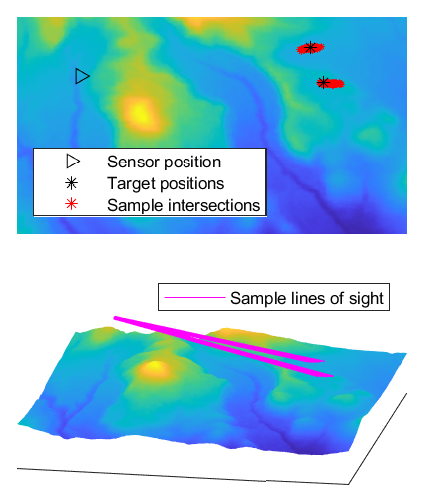
\includegraphics[scale=1.0]{TerrainTrackingExample.eps}
    \caption{In terrain-aided tracking sample lines of sight from the sensor in the direction of the target are intersected with a DEM to obtain samples from the distribution of the target positions. In this example the samples are randomly drawn from the measurement distribution, but deterministic samples (such as in the UT) can also be used.}
    \label{fig:lostrackingexample}
\end{figure}

The line of sight intersection algorithm outlined in \cite{schonborn2022terrain} will be used in the simulated scenario described in section \ref{application} and will be reviewed here briefly. For more details the reader is referred to \cite{schonborn2022terrain}. The azimuth and elevation angles from the sensor to the target are first converted into a unit vector in the corresponding direction using the standard spherical to Cartesian conversion. This yields a line of the form given in equation \ref{eq:lineofsight} where $X$ is the sensor position, $D$ is the unit vector in the direction of the target, and $t$ is a free parameter moving along the line.

\begin{equation}
\begin{aligned}
    L = {}& X + tD \\
\end{aligned} \label{eq:lineofsight}
\end{equation}

All points of intersection between $L$ and the DEM surface $X_w$ can be found by setting them equal, but the specific intersection point of interest is that which is in front of the sensor and nearest to it. Therefor $t$ can be expressed as the solution to an optimization problem, as in equation \ref{eq:losintersectionoptimization} from \cite{schonborn2022terrain}.

\begin{subequations}\label{eq:losintersectionoptimization}
\begin{alignat}{2}
&\!\min_{t}          &\qquad& t\\
&\text{subject to} &      & X + t D = X_w,\\
&                  &      & t > 0
\end{alignat}
\end{subequations}

The solution $t$ is found by traversing the DEM grid until the nearest point of intersection is reached \cite{schonborn2022terrain}. The grid tracing approach from \cite{musgrave1988grid} is used, allowing only the cells of the DEM in the path of the ray to be traversed, as shown in figure \ref{fig:gridintersection}. As the cells are traversed in order of increasing distance from the sensor, each is tested for intersection first at a coarse level with fast check on the bounding rectangular prism. If the coarse check is passed, the specific shape of the cell (a bilinear interpolation of its corner elevations) is checked for intersection using the algorithm from \cite{ramsey2004ray}. When a point of intersection is found, it will be the one nearest to the sensor (see \cite{ramsey2004ray}) and the algorithm can be stopped.

\begin{figure}[ht]
    \centering
    \includegraphics[scale=0.25]{LineGrid.png}
    \caption{DEM grid traversal along a line of sight.}
    \label{fig:gridintersection}
\end{figure}

Although the use of a DEM can improve tracking performance when simpler terrain models cannot adequately represent the terrain, they are not completely free of errors. One source of error is that the DEMs commonly used for tracking applications are limited in resolution. Computational requirements for online tracking in real time prohibit the use of DEMs with very high resolution, which can additionally are not always available for the tracking area of interest. The NASA SRTM data sets provide DEMs with resolutions of 30m \cite{jpl13} and 90m \cite{nasa00} for most of the planet, so these are reasonable resolutions to assume for practical purposes. Features of the terrain significantly smaller than the resolution of the DEM cannot be represented. The other main source of error in DEMs is elevation errors. Even large terrain features that can be seen given the resolution are not perfectly known in terms of their elevation. Figure \ref{fig:demexamples} shows the level of detail of three different publicly available DEMs (at 1m \cite{robinson2012high}, 30m \cite{jpl13}, and 90m \cite{nasa00} resolution) for the area surrounding Crater Lake, Oregon, USA.

\begin{figure}[ht]
\centering
  \begin{tabular} {@{}c@{}}
    \includegraphics[width=0.45\textwidth]{craterlake_highres_crop.png} \\
    \includegraphics[width=0.45\textwidth]{craterlake_30m_crop.png} \\
    \includegraphics[width=0.45\textwidth]{craterlake_90m_crop.png} \\
  \end{tabular}
  \caption{DEMs of the area surrounding Crater Lake at 1m, 30m, and 90m resolutions, showing the level of detail in each. Note that in this example the 1m model also includes the underwater elevation while the 30m and 90m models just include a flat surface at sea level.}
  \label{fig:demexamples}
\end{figure}

\section{Problem Formulation} \label{problemstatement}
Assume $M(k)$ targets are observed by $N(k)$ sensors at time $t_k$. For asynchronous systems (as considered here) it may be the case that $N(k) = 1$, with different sensors observing the targets at different instances in time, globally indexed by $k$. The sensors may have different measurement models, but all use a measurement model of the form given in equation \ref{eq:generalmeasurementmodel}. The notation specific to the problem is made more clear in equation \ref{eq:problemmeasurementmodel}.

\begin{equation}
    z_{s,t}^m(k) = h_s^m(x_s^m(k), x_t^m(k), \beta_s(k), v_s(k)) \\
\label{eq:problemmeasurementmodel}
\end{equation}

The measurement $z_{s,t}^m(k)$ is generated by sensor $s$ observing target $t$ at time $k$. Here $x_s^m(k)$ and $x_t^m(k)$ are the true states (in the measurement space, noted by superscript $m$) of the sensor and the target, respectively. The sensor state is included explicitly here to indicate that there may be noisy measurements that relate to the sensor as well (for example, a GPS measurement of the sensor position). Since this is already in the measurement space, the measurement model $h_s^m$ is primarily used to model how the true bias vector $\beta_{s}$ enters the measurement equation. This is not restrictive and the bias vector may contain additive (offset) and/or multiplicative (scaling) biases. The measurement noise $v_s(k)$ is assumed Gaussian zero-mean with covariance matrix $R_s(k)$, and is assumed to be independent from other noises considered.

To accommodate heterogeneous sensor models in the measurement space, the measurements are converted into Cartesian coordinates to provide a common frame of reference. In equation \ref{eq:commonreferencemeasurementmodel} the measurement conversion function $h_s^c$ is introduced, which may be highly nonlinear. The bias estimates $\hat{\beta}_s(k)$ are modelled as Gaussian random variables and are accounted for in the conversion process. These may be constant or time-varying according to some state-transition model of the form given by equation \ref{eq:generalsystemmodel}. The measurement conversion function may also depend on some additional global information $z_g$ such as road map information or terrain data (see section \ref{application} for an example). This can be considered to be constant (if known completely) or a random variable (if there is some uncertainty).

\begin{equation}
    z_{s,t}^c(k) = h_s^c(z_s^m(k), \hat{\beta}_s(k), z_g) \\
\label{eq:commonreferencemeasurementmodel}
\end{equation}

The function $h_s^c$ must map each point in the space of its input to a unique point in the state space. The converse need not be true (i.e. $h_s^c$ may be many-to-one). Note that while $z_s^m$ may contain variables referring to the sensor and the target, $z_{s,t}^c$ contains only the position of the target in the state space, which is commonly observed among all sensors. Since the converted measurements $z_{s,t}^c(k)$ depend on the bias estimates $\hat{\beta}_s(k)$ and possibly some additional information $z_g$, they cannot be considered to be uncorrelated over time. In the state space the targets are assumed to move according to a state-transition model of the form given in equation \ref{eq:generalsystemmodel}.

No particular fusion architecture is assumed. That is to say that a given fusion node may receive information about a target in the form of a measurement or a track, and received tracks may be correlated through unknown mechanisms with other tracks (such as the track at the local node). This information may be received in an asynchronous manner. Much of the discussion in sections \ref{newbiasestimation} and \ref{application} will be in the context of a distributed or decentralized network, but if the network is centralized then all information is available to reconstruct the necessary data to carry out the same operations.

Finally, it is assumed that some prior information about the bias of each sensor is available (i.e. $\hat{\beta}_s(0)$ is known). In practice this can be achieved with an initial mean of $0$ and covariance consistent with some known bounds on the bias values. This is similar to the one-point KF initialization method from \cite{bar2004estimation}. The objective is to update and refine these bias estimates, beginning with the prior, according to information obtained from multiple sensors.

For a concrete example of this type of problem formulation, see section \ref{application}.

\section{Flexible Sensor Bias Estimation} \label{newbiasestimation}
In this section a computationally efficient algorithm is proposed to estimate the measurement bias vectors in a practical scenario as described in section \ref{problemstatement} above, without adding additional assumptions that narrow the scope of application. The novelty of the proposed algorithm is that is can be applied very generally without significant restrictions in terms of the measurement model, bias model, or fusion architecture. See section \ref{application} for an example where the operational scenario does not allow the direct application of any computationally efficient method in the existing literature, but can be handled in real time by the proposed algorithm.

One important note is that in this section the data association (measurement-to-track at the local node, and track-to-track when performing fusion) will be assumed to be known. This is because the association problem is not the focus of this work. In practical applications, data association must be performed online. If some targets are poorly resolved, it may be better to use only well resolved targets in the bias estimation process. This is not ideal, so future work may be warranted to include a more rigorous consideration of data association in this context specifically.

The general strategy in the proposed algorithm can be divided into two main tasks, contained in shaded boxes in figure \ref{fig:biasestimationflowchart}. This figure  shows how an update is performed for a single target and a single sensor. The first task, in the shaded box on the left, is to maintain consistent, bias-compensated tracks for each target at each sensor node, using only locally-sourced measurements. These will be referred to as consistent local tracks. The second task, in the shaded box on the right, is to update the bias estimate. This is accomplished by forming a joint estimate between the target state and the bias estimate and updating the combined state using consistent information about the target state from other sensor nodes.

\begin{figure}[ht]
    \centering
    \includegraphics[scale=0.9]{BiasEstimationFlowchart.pdf}
    \caption{A diagram of the proposed algorithm showing the data flow for a sensor node update using a single target identified by $t$. The sensor bias estimate is updated as part of the joint estimate $\hat{x}_t^j(k)$ through cross-correlation with the target state when fusing information from other sensors.}
    \label{fig:biasestimationflowchart}
\end{figure}

The consistent local tracks are updated using CI to retain their consistency despite correlations introduced by bias compensation, without modeling these correlations explicitly (see section \ref{biascompensation} for more details on bias compensation). The consistent local tracks are sent to other sensor nodes, who fuse them all together (excluding their own track) to form a consistent non-local track that summarizes the information about the target obtained from other sensors. When an estimate for tracking output is required at the local sensor, the consistent local and consistent non-local tracks are fused to provide this. CI is used to fuse in creating both the non-local track and the tracking output because tracks from different sensors may be correlated through process noise as well as the bias compensation process.

The bias estimate update first requires forming a joint estimate of the target state and the sensor bias. This is accomplished for the instantaneous time $k$ using the UT and the two previous local measurements using the UT (the details of this are given in section \ref{utinitialization} below). This is reconstructed at every update to capture the current cross-correlations between the bias parameters and the target state directly at the instant of the update. This is required because these cross-correlations depend not only on the target state (which is tracked) but also on the sensor position (which is not tracked, but is measured). Next, the joint estimate is updated using the predicted consistent non-local track as a pseudo-measurement of sorts. Note that the joint estimate and the consistent non-local track are correlated through the bias compensation process (the bias estimates from each sensor use information from the same measurements). Because these correlations are not explicitly modeled and the non-local track does not include the bias components in the state vector, this requires information fusion under unknown cross-correlation with unequal state dimension. Several options for this are outlined in section \ref{fusionunknowncc}. Another option is to ignore the cross-correlations and use the standard KF update. This can result in inconsistent bias estimates, but there is reason to believe that the cross-correlations are small (in some sense) if the (true) bias uncertainty is small relative to the measurement uncertainty. This is because the only source of correlations is the bias compensation process. An additional alternative is proposed in section \ref{ciequivalentmeasurement}, attempting to strike a balance between some existing methods which can be too pessimistic, and the KF which can be too optimistic. Each of these options for the bias estimate update step are evaluated and compared through simulations in section \ref{application}. Since each target update yields an updated bias estimate, the updated bias estimates from each target are then fused to yield the overall updated bias estimate. Again the bias estimates from each target are correlated, so CI should be used here for the fusion.

The remainder of this section is organized as follows. Section \ref{utinitialization} describes in detail the process of forming the joint estimate between the target state and bias estimate using the UT. Section \ref{ciequivalentmeasurement} proposes a new approach for the update step with unequal state vectors under unknown cross-correlation. Section \ref{biascompensation} provides more information about the bias compensation process, and the correlations introduced by this. The proposed algorithm is given with pseudo-code in section \ref{proposedalgorithm}. An analysis of the computational complexity of the proposed algorithm is then given in section \ref{computationalcomplexity}.

\subsection{Unscented Transform for Joint Estimate Initialization} \label{utinitialization}
As described in section \ref{unscentedtransform}, the UT can be used to form a Gaussian estimate of a random variable after it undergoes a nonlinear transformation. In this section, the UT will be used to initialize a joint estimate of the stacked target state and bias estimate. This approach can be used to initialize target states using various motion models, but here an example is shown for initialization based on a constant velocity (CV) model.

First, a stacked random variable consisting of the most recent two sensor measurements, the previous bias estimate, and any additional global information is formed as in equation \ref{eq:utinputblocks}. In this example with a two-point initialization, the bias estimate from time $k-2$ is used with measurements from times $k-1$ and $k$ so that the bias estimate and the measurements are not correlated (i.e. the bias is updated once for every 2 measurements from the local sensor). The the joint distribution parameterized by $\bar{x}_{s,t}^{m,j}, P_{s,t}^{m,j}$ will be the input distribution from which the sigma points are drawn for the UT.

\begin{equation}
\begin{aligned}
    \bar{x}_{s,t}^{m,j} = {}& \begin{bmatrix}
                        \bar{z}_{s,t}^{m}(k)^{T} & \bar{z}_{s,t}^{m}(k-1)^{T} & \bar{\beta}_{s}^{T}(k-2) & 
                        \bar{z}_{g}^T \\
                    \end{bmatrix}^{T} \\
    P_{s,t}^{m,j} = {}& \begin{bmatrix}
                        R_{s}^{m}(k) & 0 & 0 & 0 \\
                        0 & R_{s}^{m}(k-1) & 0 & 0 \\
                        0 & 0 & P_{\beta}(k-2) & 0\\
                        0 & 0 & 0 & P_{g} \\
                    \end{bmatrix} \\
\end{aligned} \label{eq:utinputblocks}
\end{equation}

The transformation function $f$ is then constructed as in equation \ref{eq:utfunctioncv} to transform each of the sigma points so that the track state is initialized in a joint distribution with the bias. In this equation $\mathcal{Z}_i^m(k)$, $\mathcal{Z}_i^m(k-1)$, $\mathcal{B}_i(k-2)$, and $\mathcal{Z}_i^g$ represent components of sigma point vector $i$ (in the input space) corresponding to the most recent measurement, the previous measurement, the bias estimate, and the global information, respectively. The measurement conversion function $h_{s}^{c}$ is used to map the sensor measurements to the target position in the state space while accounting for the bias uncertainty and global information. The time index is dropped from the bias estimate to simplify the notation. It is worth reiterating here that this is the bias estimate from a time before any of the measurements used in the UT so that it is not correlated with any of them, so for a CV model this can be used every other measurement, for a constant acceleration (CA) model every third measurement, and so on. The time between the measurements is denoted $T(k, k-1)$.

\begin{equation}
\begin{aligned}
    f(\mathcal{X}_i) ={}& \begin{bmatrix}
                        \mathcal{P}_i(k) \\
                        \mathcal{V}_i(k) \\
                        \mathcal{B}_i \\
                    \end{bmatrix} \\
    \mathcal{P}_i(k) ={}& h_{s}^{c}( \mathcal{Z}_i^m(k), \mathcal{B}_i, \mathcal{Z}_i^g ) \\
    \mathcal{V}_i(k) ={}& \frac{ \mathcal{P}_i(k) - \mathcal{P}_i(k-1)}{ T(k, k-1) }
\end{aligned} \label{eq:utfunctioncv}
\end{equation}

The resulting transformed points $\mathcal{Y}_i = f(\mathcal{X}_i)$ are in the state space of the target motion model (position and velocity for a CV model) with bias augmented. These points are used to parameterize a Gaussian joint estimate of the target state and bias estimate, including the cross-correlation terms. See algorithm \ref{alg:ut} for details about drawing sigma points and the rest of the UT algorithm. For higher-order kinematic models, more measurements can be used.

\subsection{Measurement Update Equivalent to Covariance Intersection in Common State Components} \label{ciequivalentmeasurement}
The proposed algorithm involves an update step on line \ref{alg:line:updatestep} or algorithm \ref{alg:proposedmeasurementupdate} that requires information fusion under unknown cross-correlation with unequal state dimensions, as reviewed in section \ref{fusionunknowncc}. See section \ref{biascompensation} for more details about the correlations involved. In this section an alternative is proposed using the KF update with a pseudomeasurement derived according to the CI algorithm. This produces the same estimate in common state components as using the standard CI algorithm (with equal state dimensions on just the common components), while also updating the uncommon state components.

The prior estimate $\hat{x}$ will be updated with information $\hat{x}'$ to obtain the posterior estimate $\hat{x}+$, where the state components of $\hat{x}'$ are a subset of the components of $\hat{x}$. The common and uncommon state components of the estimate with the larger state can be broken down into blocks as shown in equation \ref{eq:ciequivalent_blocks}, with subscripts $c$ and $u$, respectively. The same block decomposition applies to $\hat{x}^{+}$ with the same notation.

\begin{equation}
\begin{aligned}
    \hat{x} = {}& \mathcal{N}(\bar{x}, P_{x})\\
    \bar{x} = {}& \begin{bmatrix}
                        \bar{x}_{c} & \bar{x}_{u} \\
                    \end{bmatrix}^{T} \\
    P_{x} = {}& \begin{bmatrix}
                        P_{cc} & P_{cu} \\
                        P_{uc} & P_{uu} \\
                    \end{bmatrix} \\
\end{aligned} \label{eq:ciequivalent_blocks}
\end{equation}

First, the CI estimate of the fused common state components is computed using the standard CI algorithm. This will be denoted as $\hat{x}_{ci}$ as shown in equation \ref{eq:ciequivalent_est}. This is then set equal to the posterior update of the common state components.

\begin{equation}
\begin{aligned}
    \hat{x}_{ci} ={}& CI(\hat{x}_{c}, \hat{x}', trace)\\
    \ ={}& \mathcal{N}(\bar{x}_{ci}, P_{ci})\\
    \ ={}& \hat{x}_{cc}^{+}\\
    \ ={}& \mathcal{N}(\bar{x}_{cc}^{+}, P_{cc}^{+})
\end{aligned} \label{eq:ciequivalent_est}
\end{equation}

Then, starting from the above equivalence and the Kalman Filter measurement update equations, a pseudomeasurement $z_{eq}$ with mean $\bar{z}_{eq}$ covariance $R_{eq}$ is derived. This pseudomeasurement, when used in the standard KF update, results in the same updated (fused) target state estimate as the CI algorithm does (meaning that the updated estimate of the common state is consistent if the input estimates are consistent). The derivation begins in equation \ref{eq:ciequivalent_R_1} below, where the $H$ matrix is just a selector of the common state components taking the form $H = [I 0]$.

\begin{equation}
\begin{aligned}
    P^{+} ={}& (I - P H^{T} (H P H^{T} + R_{eq})^{-1} H) P \\
    \ ={}&  (I - P H^{T} (P_{cc} + R_{eq})^{-1} H) P \\
    \ ={}&  (I - P \begin{bmatrix}
                        (P_{cc} + R_{eq})^{-1} \\
                        0_{mat} \\
                    \end{bmatrix} H) P \\
    \ ={}&  (I - \begin{bmatrix}
            P_{cc}(P_{cc} + R_{eq})^{-1} & 0 \\
            P_{uc}(P_{cc} + R_{eq})^{-1} & 0 \\
        \end{bmatrix}) P \\
\end{aligned} \label{eq:ciequivalent_R_1}
\end{equation}

Only the top-left block of the matrix from equation \ref{eq:ciequivalent_R_1}, pertaining to the common states, is required to solve for $R_{eq}$. Considering this block only after right-multiplying $P$ yields equation \ref{eq:ciequivalent_R_2}.

\begin{equation}
\begin{aligned}
    P_{ci} ={}& P_{cc} - P_{cc} (P_{cc} + R_{eq})^{-1} P_{cc} \\
\end{aligned} \label{eq:ciequivalent_R_2}
\end{equation}

Rearranging equation \ref{eq:ciequivalent_R_2} to solve for $R_{eq}$, the final expression for the covariance of the pseudomeasurement is given in equation \ref{eq:ciequivalent_R}. Note that the covariance of the estimate of the common state components must be invertible, as must be $(P_{cc}^{-1} - P_{cc}^{-1} P_{ci} P_{cc}^{-1})$.

\begin{equation}
    R_{eq} = (P_{cc}^{-1} - P_{cc}^{-1} P_{ci} P_{cc}^{-1})^{-1} - P_{cc}
\label{eq:ciequivalent_R}
\end{equation}

A similar approach is used to derive $\bar{z}_{eq}$. Again all that is required to solve for $\bar{z}_{eq}$ is the top block of equation \ref{eq:ciequivalent_z_1}, corresponding to the common state components. Considering only this block of the vector yields equation \ref{eq:ciequivalent_z_2}, which is rearranged to solve for $\bar{z}_{eq}$. The final expression for $\bar{z}_{eq}$ is given in equation \ref{eq:ciequivalent_z}.

\begin{equation}
\begin{aligned}
    \bar{x}^{+} ={}& \bar{x} + P H^{T} (H P H^{T} + R_{eq})^{-1} (\bar{z}_{eq} - H \bar{x}) \\
    \ ={}& \bar{x} + \begin{bmatrix}
            P_{cc}(P_{cc} + R_{eq})^{-1} \\
            P_{uc}(P_{cc} + R_{eq})^{-1} \\
        \end{bmatrix} (\bar{z}_{eq} - \bar{x}_{c})
\end{aligned} \label{eq:ciequivalent_z_1}
\end{equation}

\begin{equation}
    \bar{x}_{ci} = \bar{x}_{c} + P_{cc}(P_{cc} + R_{eq})^{-1} (\bar{z}_{eq} - \bar{x}_{c})
\label{eq:ciequivalent_z_2}
\end{equation}

\begin{equation}
    \bar{z}_{eq} = (I + R_{eq} P_{cc}^{-1}) (\bar{x}_{ci} - \bar{x}_{c}) + \bar{x}_{c}
\label{eq:ciequivalent_z}
\end{equation}

The measurement $z_{eq}$ is then used in the standard KF update to update the prior estimate $\hat{x}$. The posterior estimate $\hat{x}^{+}$ resulting from the update is equivalent to CI fusion in the common state components, but the estimate of the uncommon state components is also updated through correlation with the common components. In this sense $z_{eq}$ can be viewed as an approximately-decorrelated measurement under the assumption of unknown correlation between the two estimates of the common state components.

\subsection{Bias Compensation} \label{biascompensation}
Once the bias has been estimated, it can be compensated for at the measurement level. As mentioned in section \ref{introduction}, many existing works simply assume the bias estimate is good enough and adjust the measured values by the appropriate amount, and in \cite{ying20103d} it is shown that considering the variance of the bias estimate can improve tracking performance. Another important reason to consider the variance of the bias estimate is for the purpose of data association, which must be considered prior to bias estimation. If the variance of the bias estimate is not small, the measurements (and resulting tracks) may not actually be consistent with the true position of the targets. This is illustrated in figure \ref{fig:biascompensationdiagram}. The result of this can be missed or incorrect associations at the measurement or track level, in addition to reduced track accuracy. At the onset of the bias estimation process, only the prior information about the bias is known, which in the case of the proposed algorithm is assumed zero-mean with an appropriately large covariance (consistent with reasonable bias values). Therefor it is important for practical purposes to consider how bias compensation can be achieved such that both the measurements and tracks remain consistent. This discussion will assume that the bias estimate being used for compensation is consistent with the true bias.

 \begin{figure}[ht]
     \centering
     \includegraphics[scale=1.0]{BiasCompensationDiagram.pdf}
     \caption{An example comparing confidence ellipses of measurements that are unbiased, biased, and bias-compensated (with and without bias-inflation). Here the bias estimate covariance is not small relative to the measurement covariance. The measurement compensated using only the mean of the bias estimate is inconsistent with the true target position (shown with a cross), unlike the measurement that is inflated to account for the bias estimate covariance.}
     \label{fig:biascompensationdiagram}
 \end{figure}

At the measurement level, this can be handled as a part of the UT. The bias estimate can be included in the input distribution such that the sigma points generated will include bias components. Then the affects of the bias parameters can be accounted for directly according to the measurement model, prior to applying the measurement conversion. The advantage of this approach is that it is achieved without requiring any additional assumptions about the measurement conversion or bias models, only that there is a known procedure for mapping points in the joint measurement-bias space to the target position in the state space. This also lends itself well to the formation of a joint estimate including the bias (as is done in section \ref{utinitialization}). This converted measurement of the target position in the state space that accounts for bias uncertainty will be referred to as a bias-inflated measurement.

At the track level, it must be considered that the bias-inflated measurements at different times are no longer independent from one another, since they depend on the bias estimate which has been recursively updated from a previous time. Recall that in \cite{ying20103d} this is accounted for by modelling the cross-covariance terms explicitly (with some approximations). If this is not feasible for a given measurement and bias model, an alternative approach must be used. One (naive) possibility is to ignore the dependence of the bias-inflated measurements and simply use the KF to track targets. This should be less optimistic than if the variance of the bias estimate is ignored entirely in bias compensation, but is still an approximation due to the assumption of the KF that the measurements are independent from one another over time. If the bias estimate variance is small then this may be an acceptable approximation since the inflated measurements may reasonably be considered "mostly" independent. If the bias estimate variance is large (such as at the onset of the bias estimation process) it may be important to consider this correlation so that the tracks remain consistent. In this case, the cross-correlation can be treated as unknown and an approach discussed in section \ref{fusionunknowncc} can be employed for the update (such as CI). This will converge more slowly than using the KF, but can guarantee consistency and is the approach used in the proposed algorithm to maintain the consistent local tracks (as discussed in section \ref{proposedalgorithm} with reference to figure \ref{fig:biasestimationflowchart}). As the bias estimate becomes more precisely known (its variance shrinks), so does the level of correlation between bias-inflated measurements. At some point the performance trade-off (between convergence and consistency) may favor switching from updating using the assumption of unknown correlation to using that of independence.

\subsection{Proposed Bias Estimation Algorithm} \label{proposedalgorithm}
Now that the basic approach for a bias estimate update has been outlined and the preliminaries are taken care of, it is possible to describe the proposed bias estimation algorithm in detail in the form of pseudo-code. The sensor node may either make local observations of targets or receive information about targets (in the form of consistent tracks) from another sensor node. The overall bias estimation process at a single sensor node maintains the bias estimate for this sensor, as well as both a consistent local track and a consistent non-local track (summarizing information received from other sensors) for each target. The consistent non-local tracks are assumed to be from some arbitrary time in the past, noted using the time index $k-\tau$. The local sensor node may transmit its local consistent track to other sensor nodes at any time (subject to practical constraints, for example the availability of a communication channel) to be included in their (from the perspective of the other node) non-local consistent track information.

Notation is introduced here to refer to sets of variables for all targets. This notation is described in equation \ref{eq:setalltargetvariables}. Note that since these equations are now referring to a single sensor, so the subscript $s$ is dropped from the notation. The exception to this is $\hat{X}_{s}^{local}(k)$ in algorithm \ref{alg:proposedtrackupdate} where the sensor performing the update receives information from another sensor, indexed by $s$ to make it clear that this is from a different sensor node.

\begin{equation}
\begin{aligned}
    Z^m(k) ={}& \{ z_{t}^{m}(k) | t \in 1 \ldots M(k) \} \\
    \hat{X}^{local}(k) = {}& \{ \hat{x}_{t}^{local}(k) | t \in 1 \ldots M(k) \} \\
    \hat{X}^{non}(k) = {}& \{ \hat{x}_{t}^{non}(k) | t \in 1 \ldots M(k) \}
\end{aligned} \label{eq:setalltargetvariables}
\end{equation}

The bias estimate and consistent local track updates occur when local measurements are made, and this process is detailed in algorithm \ref{alg:proposedmeasurementupdate}. The inputs for this algorithm (in addition to those maintained internally, discussed above) are the measurements of each target from this time and the previous measurement time, as well as (optionally) some global information $z_g$ such as terrain data. Note that because 2 measurements are required for the update (with a CV model), this should be done only every other measurement update. When 2 measurements for a target are not yet ready, the arriving measurement can simply be queued up for the next update. If the consistent non-local track is not yet initialized, the bias update must be skipped until this is available. Similarly, targets can be skipped in the same manner if they are not associated (with local measurements or non-local tracks). On line \ref{alg:line:utinitializef} of this algorithm, the UT is used for initialization of the joint estimate between the target state and the bias vector, as described in section \ref{utinitialization}. The function $f$ used in the UT is as defined in equation \ref{eq:utfunctioncv}. On line \ref{alg:line:updatestep} of this algorithm the update operation is fusion under unknown cross-correlation with unequal state dimensions. Several alternatives to achieve this are discussed earlier in section \ref{proposedalgorithm}, and are compared through simulations in section \ref{application}.

\begin{algorithm}[H]
\caption{ProposedMeasurementUpdate\\($Z^{m}(k), Z^{m}(k-1), \hat{X}^{local}(k-2), \hat{X}^{non}(k-\tau), \hat{\beta}(k-2), z_g$)}
\label{alg:proposedmeasurementupdate}
\begin{algorithmic}[1]
\State $\hat{\beta}(k) = \hat{\beta}(k-2)$
\ForEach {$t \in 1 \ldots M(k) $}
    \LineComment{Skip targets without two measurements}
    \If {$z_{t}^{m}(k)$\ \text{or}\ $z_{t}^{m}(k-1)\ \text{not defined}$}
        \State $\text{Store}\ z_{t}^{m}(k)\ \text{for next update at time}\ k+1$
        \State \textbf{continue}
    \EndIf
    \LineComment{Initialize joint distribution (section \ref{utinitialization})}
    \State $\hat{x}_{t}^{m,j}(k) = \langle \text{Use equation \ref{eq:utinputblocks}} \rangle$
    \State $\hat{x}_{t}^{j}(k) = UT(\hat{x}_{t}^{m,j}(k), f)$ \label{alg:line:utinitializef}
    \LineComment{Update local consistent track}
    \State $\hat{x}_{t}^{state}(k) = \langle \text{Marginalize from}\ \hat{x}_{t}^{j}(k) \rangle$
    \If {$\hat{x}_{t}^{local}(k-1)\ \text{not defined}$}
        \State $\hat{x}_{t}^{local}(k) = \hat{x}_{t}^{state}(k)$
    \Else
        \State $\hat{x}_{t}^{local}(k) = \langle \text{Predict from}\ \hat{x}_{t}^{local}(k-1) \rangle$
        \State $\hat{x}_{t}^{local}(k) = CI(\hat{x}_{t}^{local}(k), \hat{x}_{t}^{state}(k), trace)$
    \EndIf
    \LineComment{Skip targets with no non-local information}
    \If {$\hat{x}_{t}^{non}(k-\tau)\ \text{not defined}$}
        \State \textbf{continue}
    \EndIf
    \LineComment{Update bias estimate}
    \State $\hat{x}_{t}^{non}(k) = \langle \text{Predict from}\ \hat{x}_{t}^{non}(k-\tau) \rangle$
    \State $\hat{x}_{t}^{j+}(k) = \langle \text{Update} \ \hat{x}_{t}^{j}(k)\ \text{with}\  \hat{x}_{t}^{non}(k) \rangle$ \label{alg:line:updatestep}
    \State $\hat{\beta}_{t}(k) = \langle \text{Marginalize from}\ \hat{x}_{t}^{j+}(k) \rangle$
    \State $\hat{\beta}(k) = CI(\hat{\beta}(k), \hat{\beta}_{t}(k), trace)$
\EndFor
\State \textbf{return} $\hat{\beta}(k), \hat{X}^{local}(k)$
\end{algorithmic}
\end{algorithm}

The consistent non-local tracks are updated or initialized when tracks are received from another sensor, as described in algorithm \ref{alg:proposedtrackupdate}. Here the inputs are the consistent non-local track (maintained from the previous time step) and the consistent local track from arbitrary other sensor node identified by $s$. Note that for the latter, this is "local" from the perspective of sensor $s$, not the sensor being updated. The local measurement information from the sensor being updated is intentionally excluded from the consistent non-local track.

\begin{algorithm}[H]
\caption{ProposedTrackUpdate($\hat{X}^{non}(k-\tau), \hat{X}_{s}^{local}(k)$)}
\label{alg:proposedtrackupdate}
\begin{algorithmic}[1]
\ForEach {$t \in 1 \ldots M(k) $}
    \LineComment{Initialize non-local consistent track for new targets}
    \If {$\hat{x}_{t}^{non}(k-\tau)\ \text{not defined}$}
        \State $\hat{x}_{t}^{non}(k) = \hat{x}_{s,t}^{local}(k)$
    \LineComment{Update non-local consistent track for existing targets}
    \Else
        \State $\hat{x}_{t}^{non}(k) = \langle \text{Predict from}\ \hat{x}_{t}^{non}(k-\tau) \rangle$
        \State $\hat{x}_{t}^{non}(k) = CI(\hat{x}_{t}^{non}(k), \hat{x}_{s,t}^{local}(k), trace)$
    \EndIf
\EndFor
\State \textbf{return} $\hat{X}^{non}(k)$
\end{algorithmic}
\end{algorithm}

These updates may happen at any time in a practical system, depending which information arrives when, calling the appropriate update function for the incoming information. The proposed algorithm requires data about a shared target from at least one non-local sensor in order to update the bias estimates, so can only be applied in scenarios with at least two sensors, but has no upper limit on the number of sensors. When online tracking output is required, the consistent tracks (local and non-local) maintained during bias estimation are fused for each target using CI to account for all available information and predicted to the current time. Alternatively, the tracking can be considered separately from bias estimation and this information can be bias-compensated and fused in a standard way as it arrives.

\subsection{Computational Complexity} \label{computationalcomplexity}
The proposed algorithm is intended for online use, so it is essential to have manageable computational requirements. This section will first consider the basic operations that dominate the computational load, which for this algorithm will be matrix inversion and finding the square root of a matrix. Next, the two major existing algorithms used in the proposed algorithm (CI and the UT) will be discussed in terms of their use of these dominating basic operations. Finally these will be placed in the context of the proposed algorithm to assess its overall computational complexity.

Inversion of an $n$-by-$n$ matrix is often considered to have computational complexity $\mathcal{O}(n^3)$. Although asymptotically-faster algorithms exist to invert a matrix as fast as $\mathcal{O}(n^{2.373})$ \cite{williams2012multiplying}, they have large constant factors that can prohibitive for practical applications unless $n$ is very large \cite{smirnov2013bilinear}. For this discussion the computational complexity of matrix inversion will be considered to be cubic, though the real-time practical considerations would still apply if a near-quadratic algorithm were discovered. The complexity of finding the square root of an $n$-by-$n$ matrix is also $\mathcal{O}(n^3)$ \cite{higham1987computing}.

Matrix inversion is the dominating factor of the computational complexity of the CI algorithm. In general for CI a constrained optimization problem must be solved to minimize the cost function which is (typically) a function requiring inversion (see algorithm \ref{alg:ci}). The proposed algorithm uses the trace of the fused matrix as a cost function, and solves this optimization problem using the bisection method, requiring a constant number of matrix inversions (assuming the required precision to be constant). Therefor the computational complexity of the CI algorithm to fuse two $n$-by-$n$ matrices is also $\mathcal{O}(n^3)$. It is worth noting that the computational complexity of standard KF update is also $\mathcal{O}(n^3)$, but with smaller constants since solving an optimization problem is not required.

The UT involves finding the square root of the input covariance matrix, but also involves the transformation of each sigma point according to the function $f$ (see algorithm \ref{alg:ut}). The UT in general and does not specify what the function $f$ is, so is must be considered as a variable factor. Therefor the computational complexity of the UT for an input matrix of size $n$-by-$n$ is $\mathcal{O}(n^3 + nf)$.

The proposed non-local consistent track update (algorithm \ref{alg:proposedtrackupdate}) is effectively a standard application of the CI algorithm. The track update is performed whenever information is received from other sensors. This must of course be performed for each target, with the number of targets denoted in this section without a time index as $M$. The information being fused is the target state, its dimension denoted in this section as $n_{x}$. Accordingly, the computational complexity of this operations for all targets for each update is given in equation \ref{eq:ccproposedtrackupdate}. For most practical applications using kinematic models to track non-cooperative targets, this state vector does not get particularly large. For example, using a constant velocity model in 3 dimensions the dimension of the target state vector will be 6. In any case, this is similar to a standard tracking application (without bias estimation) and computational demands at least similar to this must be expected when fusing information from other sensors.

\begin{equation}
\begin{aligned}
    \mathcal{O}(ProposedTrackUpdate) ={}& \mathcal{O}(M n_{x}^3) \\
\end{aligned} \label{eq:ccproposedtrackupdate}
\end{equation}

The proposed measurement update (algorithm \ref{alg:proposedmeasurementupdate}) is where the bias estimation actually happens and involves both CI and the UT, as well as an update step which also must be considered. CI is used to update both on the local consistent track (state vector of dimension $n_{x}$), as well as the bias estimate. The dimension of the bias vector will be referred to as $n_{\beta}$. The UT is performed here on the joint distribution created by stacking two measurements and the bias vector (see section \ref{utinitialization}). The dimension of the measurement vector will be denoted $n_{m}$, so the dimension of the joint distribution that is input to the UT is $2n_{m} + n_{\beta}$. The update step, line \ref{alg:line:updatestep} of this algorithm, can be achieved in several ways (see section \ref{application} for a comparison). This is a fusion with unequal state dimension where a joint distribution between the target state and bias vector (dimension $n_{x} + n_{\beta}$) is updated with information about the target state (dimension $n_{x}$). The computational complexities of each of these update methods (compared through simulation in section \ref{application}) is dominated again by matrix inversion in the dimension of this joint state. Each of these operations is required for each target used in the update. Putting this all together, the computational complexity of the proposed measurement update is given in equation \ref{eq:ccproposedmeasurementupdate}.

\begin{multline}
    \mathcal{O}(ProposedMeasurementUpdate) =\\
    \mathcal{O}(M((n_{m} +n_{\beta})^3 + (n_{m} +n_{\beta})f + (n_{x} + n_{\beta})^3))
\label{eq:ccproposedmeasurementupdate}
\end{multline}

What is important to notice is that neither of the complexities in equations \ref{eq:ccproposedtrackupdate} or \ref{eq:ccproposedmeasurementupdate} depend directly on the number of sensors (denoted in this section without a time index as $N$). This only comes into play in how frequently algorithm \ref{alg:proposedtrackupdate} is called. In some sense, this could be considered linear in the number of sensors if the number of sensors are constant over time and all report information regularly, although the proposed algorithm does not assume this to be the case. It is also important that both of these algorithms depend only linearly on the number of targets. The terms involving $f$ resulting from the use of the UT are difficult to compare due to the very general nature of the approach, but if $f$ is fast to evaluate this will not be an issue.

Compare this to the full form of the ASKF operating on sensors with uniform measurement and bias models, which is a standard KF with computational complexity dominated by matrix inversion. The full ASKF uses a state vector of dimension $M n_{t} + N n_{\beta}$, so it has a much larger asymptotic complexity of $\mathcal{O}((M n_{t} + N n_{\beta})^3)$, which cubic both in the number of targets and in the number of sensors. Even more computationally-friendly approaches (such as the pseudo-measurement approach) usually involve a stacked state vector that grows with the number of sensors (or the approach is limited to two sensors), resulting in complexity cubic in the number of sensors but linear in the number of targets. This makes the proposed algorithm much more computationally efficient for scenarios with a large number of sensors.

Since tracking is also performed online, its computational complexity is also important to consider. The proposed algorithm can be used in a standard tracking framework with the bias-compensated converted measurements filtered using a KF and non-local tracks fused using a standard application of the CI algorithm. Alternatively, the local consistent track and non-local consistent tracks, which are already being maintained for bias estimation purposes, can be fused using the standard CI algorithm. In either case, the computation of the updates for tracking output are dominated again by matrix inversion, with complexity cubic in the size of the state vector and linear in the number of targets.

\section{Simulations} \label{application}
To evaluate the proposed algorithm and demonstrate its effectiveness and flexibility, simulations were conducted for an application to terrain-aided tracking using video sensors. The proposed algorithm for bias estimation and compensation is compared against tracking with unbiased measurements, and with bias-ignorant measurements (subject to bias that is ignored when tracking). These comparisons serve as high and low baselines, respectively. Several approaches for fusion under unknown cross-correlation with unequal state vectors (applied in the context of the proposed algorithm) are also compared, as well as the different approaches to bias compensation outlined in section \ref{biascompensation}. Two approaches to bias-compensated tracking are compared as well. In the first, a standard KF is used to track with the bias-compensated converted measurements. This first approach ignores some sources of correlation over time between the measurements (more details are given in sections \ref{biascompensation} and \ref{applicationmeasurementmodels}). These are based only on local measurements at each sensor node and the bias estimates. The second approach is to fuse the consistent local track and the consistent non-local track, maintained already by each sensor node for the purposes of bias estimation, using CI. This accounts for the correlations between the tracks while utilizing all the information available to the sensor node. For performance evaluation purposes 500 Monte Carlo runs were conducted. Estimation accuracy in both bias estimates and bias-compensated tracks are evaluated using the Root Mean Square Error (RMSE) metric. Track consistency is evaluated using chi-square tests on Average Normalized Estimation Error Squared (ANEES) metric.

\subsection{Scenario} \label{applicationscenario}
In each Monte Carlo run the true target and sensor trajectories are regenerated randomly according to their process noises and (static) initial conditions, and the true sensor biases (constant over a single run) are drawn from a distribution consistent with the bias prior. Targets move according to a 2-dimensional nearly constant velocity (NCV) model with their elevation fixed to the ground, while sensors move through the air according to a nearly constant acceleration (NCA) model. Both of these models are described in detail in \cite{bar2004estimation}. Based on the trajectories, bias, and measurement noise distributions, noisy sensor measurements are generated randomly for each run and these are used to estimate the sensor biases and target states.

A distributed fusion architecture with 4 sensors observing 4 targets is considered. The sensors take measurements at a rate of 10 frames per second for a period of 300 seconds. Each sensor measures their own position in 3 dimensions as well as the azimuth and elevation angles to each target, subject to Gaussian zero-mean measurement noise. The measurement noise standard deviations were set to 0.5 degrees for the angular components and 3 meters for the positional components. In addition to the zero-mean noise, the angular measurements are also subject to additive constant biases. The bias prior for the angular components is zero-mean with a standard deviation of 2 degrees. The targets are tracked using a 3-dimensional NCV model, as described in \cite{bar2004estimation}. At each time step the sensors communicate their tracks to one another after updating their local tracks and bias estimates. This is to mimic the realistic condition that sensors cannot communicate this information instantaneously, and the effect is that when sensor nodes are performing their local update they have access to information from other nodes only from the previous time step. To illustrate the ability of the proposed algorithm to function in a fully distributed scenario with unreliable communication, simulation results are also presented for a scenario where each sensor only has a 50\% chance to receive information from each other sensor at every time step.

\subsection{Digital Elevation Models} \label{applicationdems}
Two DEMs were used in the simulated scenario. The first, a high resolution DEM with a resolution of 1m (from \cite{robinson2012high}), was used to simulate realistic true trajectories for ground targets. The second, a DEM with a resolution of 30m (from \cite{jpl13}), was used during tracking. DEMs at a 30m resolution are generally available for most locations around the world \cite{jpl13} and they are computationally feasible for use in real time. The level of detail of each of these DEMs can be seen in figure \ref{fig:demexamples}. The differences between these two DEMs mimic realistic terrain elevation errors when tracking.

\subsection{Measurement Models for Terrain-Aided Tracking} \label{applicationmeasurementmodels}
The measurement model $h_{s}^{m}$ of the form in equation \ref{eq:problemmeasurementmodel}, defining how the true additive bias affects the measurement, is given below in equation \ref{eq:applicationmeasurementmodel}.

\begin{equation}
\begin{aligned}
    z_{s,t}^m(k) ={}& h_s^m(x_s^m(k), x_t^m(k), \beta_s, v_s(k)) \\
    \ ={}& \begin{bmatrix}
            x_{s,x}(k) \\
            x_{s,y}(k) \\
            x_{s,z}(k) \\
            x_{t,az}(k) \\
            x_{t,el}(k)
        \end{bmatrix} + \begin{bmatrix}
            0 \\
            0 \\
            0 \\
            \beta_{az} \\
            \beta_{el}
        \end{bmatrix} + v_s(k) \\
    \ ={}& \bar{z}_{s,t}^{m}(k) + v_s(k) \\
    \ ={}& \mathcal{N}(\bar{z}_{s,t}^{m}(k), R_s(k))
\end{aligned} \label{eq:applicationmeasurementmodel}
\end{equation}

The measurement conversion model is applied to transform the measurement $z_{s,t}^m(k)$ and bias estimate to a converted bias-compensated measurement in the target state space. Here the global information $z_g$ is a one-dimensional zero-mean Gaussian noise used to represent the terrain uncertainty. The UT is used here with the joint distribution consisting of the measurement, bias estimate, and global information as input. The nonlinear transformation $h_s^c$ will be applied to the sigma points as in equation \ref{eq:applicationmeasurementconversionmodel}.

\begin{equation}
\begin{aligned}
    z_{s,t}^c(k) ={}& h_s^c(z_s^m(k), \hat{\beta}_s(k), z_g) \\
    \mathcal{Z}_i^c(k) ={}& h_{s}^{c}( \mathcal{Z}_i^m(k), \mathcal{B}_i(k), \mathcal{Z}_i^g )
\end{aligned} \label{eq:applicationmeasurementconversionmodel}
\end{equation}

First, bias-corrected sigma points $\mathcal{Z}_i^{m,bc}$ in the measurement space are computed by subtracting the bias components from the corresponding measurement components of each sigma point, as in equation \ref{eq:biascompensationsigma}.

\begin{equation}
\begin{aligned}
    \mathcal{Z}_i^{m,bc}(k) ={}& \begin{bmatrix}
            \mathcal{Z}_{i,s,x}^m \\
            \mathcal{Z}_{i,s,y}^m \\
            \mathcal{Z}_{i,s,z}^m \\
            \mathcal{Z}_{i,t,az}^m \\
            \mathcal{Z}_{i,t,el}^m
        \end{bmatrix} - \begin{bmatrix}
            0 \\
            0 \\
            0 \\
            \mathcal{B}_{i,az} \\
            \mathcal{B}_{i,el}
        \end{bmatrix}\\
\end{aligned} \label{eq:biascompensationsigma}
\end{equation}

Next, each representing a possible line of sight from the sensor to the target, these bias-corrected sigma points are transformed to the state space by calculating its point of intersection with the tracking DEM. This is expressed in equation \ref{eq:biascompensatedintersectionpoint}.

\begin{equation}
\begin{aligned}
    \mathcal{Z}_i^{c}(k) ={}& IntersectionPoint(\mathcal{Z}_i^{m,bc}(k), DEM, \mathcal{Z}_i^g)
\end{aligned} \label{eq:biascompensatedintersectionpoint}
\end{equation}

The DEM intersection algorithm described in \cite{schonborn2022terrain} is used to compute $\mathcal{Z}_i^{c}$ (see section \ref{terrainaidedtracking}). The final argument to the function in equation \ref{eq:biascompensatedintersectionpoint} is the sigma point component $\mathcal{Z}_i^g$, corresponding to the DEM elevation error. When each point of intersection between the line of sight $\mathcal{Z}_i^{m,bc}$ and the DEM is calculated, the entire DEM is offset by adding $\mathcal{Z}_i^g$ to its elevation values. This simplified error model for the DEM is used to retain computational efficiency without ignoring the errors entirely. Note that here the converted measurements are not uncorrelated over time due to the uncertainty introduced by the DEM.

\subsection{Algorithm and Scenario Variation Nomenclature}
The algorithm proposed in section \ref{proposedalgorithm} leaves several options open in terms of the joint estimate update used to refine the bias estimate. The identifier used for each algorithm variation will correspond to the method used in the update step, where the standard Kalman Filter, the method proposed in section \ref{ciequivalentmeasurement}, Covariance Intersection (with unequal state dimension) from \cite{uhlmann1995dynamic}, and Covariance Bounds from \cite{noack2014fusion} will be considered. The abbreviations KF, CIKF, CI, and CB will be used, respectively, to identify these variations. These algorithms will also be compared with the standard KF applied to unbiased measurements (as a high performance baseline) and biased measurements without any bias compensation (as a low performance baseline). These baseline approaches will be identified by UB and BI, respectively. In addition to different algorithm variations, two scenarios are considered, one with full communication and one with limited communication, as outlined in section \ref{applicationscenario}. The identifiers for these scenarios will be FC and LC, respectively. For example, results presented that use the standard Kalman Filter for the joint estimate update under full communication will be labelled KF-FC.

\subsection{Results} \label{simulationresults}
Bias estimation is the primary focus of this work and it is of course important that the proposed approach can produce accurate bias estimates. Figure \ref{fig:resultsbiasrmse} shows a plot of the RMSE of the bias estimates (Euclidean distance error) over time for each of the algorithm and scenario variations. Similar trends are visible in each sensor with the lowest RMSE coming from the CIKF update, followed closely by the KF update, and then the CI update. In each case, the LC scenarios have slightly higher error than the corresponding FC scenarios. This difference between the scenarios is slightly more pronounced in the CI update algorithm variation.

\begin{figure}[ht]
    \centering
    \includegraphics[scale=0.85]{bias_rmse.pdf}
    \caption{Root Mean Square Error (RMSE) for the bias estimates $\hat{\beta}_{s}$ for each sensor $s$.}
    \label{fig:resultsbiasrmse}
\end{figure}

In these simulations the data association has been assumed to be known, but in a real world application the converted bias-compensated measurements and the local consistent track from each sensor will need to be associated with one another during the bias estimation process. If this data association is to be performed reliably, both of these should be consistent estimates. This is verified using chi-square tests on the ANEES metric. The one-sided chi-square test is used here due to its similarity with the standard gating process used in data association. Figures \ref{fig:resultsmeasurementaneess1t1} and \ref{fig:resultslocaltrackaneess1t1} show the results of these tests for the converted bias-compensated measurements and the local consistent tracks, respectively, for a single sensor and a single target. Nearly all of the time the ANEES is within the shaded 95\% acceptance region, indicating that both are consistent estimates.

\begin{figure}[ht]
    \centering
    \includegraphics[scale=0.85]{measurement_anees_s1t1.pdf}
    \caption{Average Normalized Estimation Error Squared (ANEES) for the converted bias-compensated measurements $z_{1,1}^{c}$, with the chi-square test acceptance region shaded.}
    \label{fig:resultsmeasurementaneess1t1}
\end{figure}

\begin{figure}[ht]
    \centering
    \includegraphics[scale=0.85]{localtrack_anees_s1t1.pdf}
    \caption{Average Normalized Estimation Error Squared (ANEES) for the local consistent tracks $\hat{x}_{1,1}^{local}$, with the chi-square test acceptance region shaded.}
    \label{fig:resultslocaltrackaneess1t1}
\end{figure}

In addition to bias estimation performance, it is also important to consider the performance of bias-compensated tracking in terms of both accuracy and consistency. Perhaps the simplest approach is to use the standard KF framework operating on the converted bias-compensated measurements originating from local sensor node. Figure \ref{fig:resultskftrackrmses1t1} shows a plot of the RMSE of these tracks for a single sensor and target, including the unbiased and bias-ignorant trackers as a baseline. A logarithmic scale here is used due to the substantially higher RMSE of the bias-ignorant tracks. The lowest RMSE among the bias-compensated tracks comes from the algorithm variation using the CIKF update, followed closely by the KF variation, and then the CI variation. Similar to what was seen in the RMSE of the bias estimates, the LC scenarios have slightly higher error than the corresponding FC scenarios, with a slightly more pronounced difference between the two in the CI variation. Bias-compensated tracks using any of the proposed algorithm variations are significantly more accurate than the bias-ignorant tracks, and those using the KF and CIKF variations converge to a level of track accuracy comparable to the unbiased tracks.

\begin{figure}[ht]
    \centering
    \includegraphics[scale=0.85]{kftrack_rmse_s1t1.pdf}
    \caption{Root Mean Square Error (RMSE) plotted on a logarithmic scale for the tracks from standard KF operating on bias-compensated measurements $z_{1,1}^c$.}
    \label{fig:resultskftrackrmses1t1}
\end{figure}

Notice that track that was bias-compensated according to the bias estimates from CIKF update algorithm actually outperforms the unbiased tracker by the end of the simulation period. The unbiased tracker is included as a high performance baseline, so this at first glance seems unexpected and must be explained. As previously noted, this application violates the assumptions of the KF that the measurement noise is zero-mean and independent over time (see sections \ref{biascompensation} and \ref{applicationmeasurementmodels}). This can lead the filter to be inconsistent, optimistic in the accuracy of its estimates. This optimism is seen clearly in figure \ref{fig:resultskftrackaneess1t1}, showing the chi-square test results for these tracks. The ANEES metric quickly exceeds the 95\% acceptance region for all trackers, even the unbiased tracker. The bias-compensated measurements have inflated covariance relative to the unbiased measurements, partially mitigating the optimism, but this is not a proper solution. Since the KF and CIKF algorithm variations have ANEES values that converge to levels comparable to those of the unbiased tracker, the majority of the dependence over time seems to be due to the terrain errors. Modelling the terrain errors more accurately as a time-varying (location-dependent) bias specific to individual targets may be a more appropriate solution, and this may be a fruitful avenue for future work.

\begin{figure}[ht]
    \centering
    \includegraphics[scale=0.85]{kftrack_anees_s1t1.pdf}
    \caption{Average Normalized Estimation Error Squared (ANEES) for the tracks from standard KF operating on bias-compensated measurements  $z_{1,1}^c$, with the chi-square test acceptance region shaded.}
    \label{fig:resultskftrackaneess1t1}
\end{figure}

The standard KF cannot be expected to produce consistent tracks with measurements that are not independent over time unless this dependence is explicitly accounted for. In general this may not always be possible, and indeed this problem seems likely to occur in practically all real world non-cooperative tracking applications that rely on an imperfect terrain model. As seen in the local consistent tracks, using CI to update the tracks instead of the KF allows for the tracks to be maintained in a consistent way, as long as the measurements or tracks to be fused are each consistent themselves. This consistency is not obtained without a price however, the estimation accuracy may suffer. This can be seen by comparing the RMSE of the local consistent tracks, shown in figure \ref{fig:resultslocaltrackrmses1t1}, with that of the standard KF tracks, shown in figure \ref{fig:resultskftrackrmses1t1}. Both of these tracks use the same measurements and bias estimates, and the tracking methods show a trade-off between consistency and accuracy.

\begin{figure}[ht]
    \centering
    \includegraphics[scale=0.85]{localtrack_rmse_s1t1.pdf}
    \caption{Root Mean Square Error (RMSE) plotted on a logarithmic scale for the local consistent tracks $\hat{x}_{1,1}^{local}$.}
    \label{fig:resultslocaltrackrmses1t1}
\end{figure}

The local consistent tracks mentioned in the above comparison are used during bias estimation and are not intended to be used directly as tracker output, so their consistency is prioritized over their accuracy. If the consistent local tracks $\hat{x}_{s,t}^{local}$ and the consistent non-local tracks $\hat{x}_{s,t}^{nonlocal}$ (already maintained during bias estimation) are fused using CI then a more accurate track can be produced that remains consistent. Examining the RMSE of these fused tracks in figure \ref{fig:resultsfusedtrackrmses1t1} reveals that they are similarly accurate to the tracks from the standard KF tracker, although they do not decrease as smoothly. The chi-square test on the ANEES of these tracks confirms that they are also consistent, as seen in figure \ref{fig:resultsfusedtrackaneess1t1}.

\begin{figure}[ht]
    \centering
    \includegraphics[scale=0.85]{fusedtrack_rmse_s1t1.pdf}
    \caption{Root Mean Square Error (RMSE) plotted on a logarithmic scale for the tracks obtained by fusing the local consistent tracks $\hat{x}_{1,1}^{local}$ and non-local consistent tracks $\hat{x}_{1,1}^{nonlocal}$ using CI.}
    \label{fig:resultsfusedtrackrmses1t1}
\end{figure}

\begin{figure}[ht]
    \centering
    \includegraphics[scale=0.85]{fusedtrack_anees_s1t1.pdf}
    \caption{Average Normalized Estimation Error Squared (ANEES) for the tracks obtained by fusing the local consistent tracks $\hat{x}_{1,1}^{local}$ and non-local consistent tracks $\hat{x}_{1,1}^{nonlocal}$ using CI, with the chi-square test acceptance region shaded.}
    \label{fig:resultsfusedtrackaneess1t1}
\end{figure}

The data so far has been presented for only sensor 1 and target 1 to show a high level of detail, but similar results are seen across all sensors and targets. To demonstrate this, the RMSE of the standard KF tracks, local consistent tracks, and fused tracks for all sensors and targets are included in figures \ref{fig:resultskftrackrmse}, \ref{fig:resultslocaltrackrmse}, and \ref{fig:resultsfusedtrackrmse}, respectively. Unlike the more detailed plots, a linear scale is used here to provide a more intuitive understanding of the differences between the various tracks. ANEES plots for all sensors and all targets are omitted for brevity.

\begin{figure}[ht]
    \centering
    \includegraphics[scale=0.85]{kftrack_rmse.pdf}
    \caption{Root Mean Square Error (RMSE) for the tracks from standard KF operating on bias-compensated measurements $z_{s,t}^c$.}
    \label{fig:resultskftrackrmse}
\end{figure}

\begin{figure}[ht]
    \centering
    \includegraphics[scale=0.85]{localtrack_rmse.pdf}
    \caption{Root Mean Square Error (RMSE) for the local consistent tracks $\hat{x}_{s,t}^{local}$.}
    \label{fig:resultslocaltrackrmse}
\end{figure}

\begin{figure}[ht]
    \centering
    \includegraphics[scale=0.85]{fusedtrack_rmse.pdf}
    \caption{Root Mean Square Error (RMSE) for the tracks obtained by fusing the local consistent tracks $\hat{x}_{s,t}^{local}$ and non-local consistent tracks $\hat{x}_{s,t}^{nonlocal}$ using CI.}
    \label{fig:resultsfusedtrackrmse}
\end{figure}

\section{Discussion} \label{discussion}

The simulation results presented in section \ref{simulationresults} demonstrate that the proposed algorithm can effectively estimate sensor biases, particularly the algorithm variations using KF and CIKF for the bias estimate update. The bias estimates from these variations can be used to reduce the bias-compensated track RMSE to levels comparable to those of a tracker operating on unbiased measurements while using a standard KF tracking framework. Although the tracks obtained from the standard KF are not consistent due to the converted bias-compensated measurements not being zero-mean or independent over time, this effect is also observed in the unbiased tracker and is primarily a result of imperfectly-known terrain. If the proposed algorithm is used in other applications that do not involve terrain models (for example, in stereo video or radar applications) this may be less of an issue. For the application at hand, this lack of consistency is resolved while retaining a similar level of track accuracy by fusing the consistent local and non-local tracks that are already maintained for the purposes of bias estimation. The simulations are done in the context of a distributed fusion architecture with unreliable asynchronous communication, using angle-only measurements taken from a sensor platform with location uncertainty, and a nonlinear terrain-aided measurement conversion model to track targets through varied terrain in real time. This is a challenging operational scenario that cannot be handled by existing computationally-efficient bias estimation approaches without significant modification, and was chosen to showcase the flexibility afforded by the proposed approach. Although not directly demonstrated through simulation, the proposed algorithm can also handle heterogeneous sensor models, networks with a large number of sensors, time-varying biases, and other fusion architectures. This flexibility allows bias estimation to be applied with minimal modification in combination with various tracking techniques and under operational conditions where it was not previously possible. This bridges an important gap in practical tracking applications.

%The issue of consistency has been a central focus of much existing work in the area of bias estimation and the field of multisensor-multitarget tracking in general. Widely considered an important quality of an estimator, proof or empirical demonstration of consistency is frequently sought. However, this is often given in the context of assumptions which may not hold up in the real world, such as flat, perfectly-known terrain. The results seen here underscore the need to develop realistic scenarios in theories and and in simulations when assessing the performance of estimators. Additional considerations and trade-offs may need to be considered when these estimators are used in practical applications.

It is important to mention that the proposed algorithm is not without limitations. The most pressing limitation is that it is not theoretically optimal. Various correlations are assumed to be unknown during the bias estimation process, or are neglected in some algorithm variations. Some notion of optimality could be chased by explicitly modelling these correlations, but this would require non-negligible effort that would be necessarily application-specific. Such an approach would come at the expense of flexibility and probably additional computational demands. It is also worth noting that even if this expense is paid, optimality is likely to only be achieved under stringent assumptions that are unlikely to hold up strictly in the real world. It is for this reason that the proposed approach eschews an optimal solution in favor of one that is flexible.

Another related limitation of the proposed algorithm is that none of the options for performing the joint estimate update to update the bias estimate are necessarily ideal, even under the assumption of unknown correlations. As seen in the simulation results, they can yield varied results. These approaches and their limitations have been discussed already in section \ref{fusionunknowncc} and \ref{ciequivalentmeasurement}. This is already a problem that is an area of active research, but future developments here may lead to direct improvements in the performance of the proposed algorithm if they can be effectively applied to it.

In terms of bias-compensated tracking, another limitation is that the two approaches presented in simulations here are two extremes. The standard KF framework assumes measurement noise to be entirely independent over time, while updating using CI exclusively assumes the correlation over time to be entirely unknown. In reality, the measurement noise originating from the sensors directly is independent over time, but the uncertainty introduced by the terrain conversion and bias compensation processes is not. Hybrid approaches that take advantage of this (such as Split Covariance Intersection (SCI), originally proposed in \cite{julier2007using}) have been applied to similar situations. If the independent and dependent components of the measurements can be effectively separated, this may provide a path for improvement. This could also possibly be applied to the maintenance of the consistent local and non-local tracks used in bias estimation, which may improve performance not only of tracking but also of bias estimation.

\section{Conclusion} \label{conclusion}
In multisensor-multitarget tracking applications sensor biases that are not compensated for can result in significantly degraded performance. This can take the form of decreased track accuracy, decreased track probability of detection, formation of ghost tracks, or missed associations. In light of this, bias estimation and compensation are essential for practical applications where it is often difficult to ensure that there are no sensor biases present. Despite a significant body of literature on the subject, existing computationally-efficient approaches remain tied to specific assumptions about the operational conditions such as particular fusion architectures, communication network properties, sensor types, measurement models, terrain configurations, constant or time-varying biases, or number of sensors.

The algorithm proposed here is one that is generally applicable to a wide range of scenarios, and here lies its novelty. It is formulated by restructuring the estimation problem so that virtually any shared state information about a target can be used to update the bias estimates. By compiling state information about a single target from other sensor nodes using the CI algorithm a consistent summary of this information is maintained that can be used to update the local sensor's bias estimate through correlation with the common target state components. The UT is used to form a joint estimate of the target state and bias estimate, and the summarized state information from other sensors is then used to update the joint state. Although the problem is restructured to minimize the degree of correlation between the joint estimate and the track summary, it is not completely eliminated. Therefor the update step requires fusion under unknown correlation with unequal state dimensions, which remains an area of active research interest. Several options for accomplishing this are explored through simulations, and this may be an area where further improvements are possible. Despite the fact that each of these options are imperfect, the proposed algorithm is shown in a challenging simulated scenario to estimate the sensor biases effectively. The corresponding bias-compensated measurements can be used in a standard KF tracking framework yielding tracks that are comparable to those of a tracker operating on unbiased measurements in terms of accuracy and consistency. In the demonstrated scenario, even the unbiased tracker is inconsistent due to the dependence of the converted measurements over time. Consistent and comparably accurate tracks are obtained by fusing the consistent local and non-local tracks already being maintained for the purpose of bias estimation. This flexible approach allows for sensor biases to be effectively estimated and compensated for in real time under practical operational conditions and with various tracking approaches where it was not previously possible to do so.

%\tableofcontents

\bibliographystyle{IEEEtran}
\bibliography{references}
\end{document}


